\section{Experiments}

We present various mathematical expressions which can be computed more efficiently
than the initial formulation would suggest. 

\subsection{Matrix Multiplication-Sum Identities}

Given matrices $A \in \mathbb{R}^{n \times m}$, $B \in \mathbb{R}^{m
  \times k}$, we wish to compute:
\begin{gather*}
\sum AB = \sum_{i = 1}^n \sum_{k = 1}^m \sum_{j = 1}^k A_{i, k} B_{k, j} 
\end{gather*}
A naive algorithm would take $O(nmk)$ time. However, we have found with our framework 
computation giving the same expression in $O(n(k + m))$ time:
\begin{lstlisting}
sum(sum(A .* repmat(sum(B, 2), [1, m])'))
\end{lstlisting}
Empirical tests indicate that our expression is indeed faster to
compute than the naive one (see Figure \ref{ab}).

Similarly, we found quadratic time computation, instead of cubic, for
similar expressions such as: 
\begin{align*}
	\sum ABC\text{, }\sum AA^T\text{, }\sum AA^TA
\end{align*}

As far we we are aware, these identities appear to be novel. Our
system could automatically analyze large code repositories to find
these and other expressions, which are currently computed
inefficiently. Alternatively, our optimization rules could be placed
into compilers to generate efficient code.

\subsection{Partition Function Approximation}

As we showed in Section \ref{partitionfunction}, we can manually find
$O(n^2)$ computation of $g(x \rightarrow x^k, W)$ for $k = 1, 2$
instead of native exponential time computation. By use of our
framework, we found rules for $k = 3, 4, 5, 6$. However for $k = 4, 5, 6$
these rules used computation with $O(n^3)$ time (i.e.~matrix
multiplication). Finding computational rules for higher degree
polynomials is expensive: Table \ref{grammars} shows the time
necessary to generate all the rules. Note that the grammar
need only be evaluated once, with the resulting coefficients being
stored. Furthermore, the process of discovering the computational rule
for a given power also need only be performed once. However, due to limited computational
power we were able to analyze powers $k \leq 6$. As we note in Section
\ref{subsec:agenda}, a future direction would be to learn patterns for
$k=2, 3, 4, 5, 6$ that allow us to generalize to $k>6$ without exhaustively
searching all possible rules. 
Table \ref{eval} shows number of terms necessary to derive $g(x
\rightarrow x^k, W)$ for various $k$. Figure \ref{approximations}
shows how well partition function is approximated with finite Taylor
expansion. Figure \ref{error_approx} shows the approximation error of
the Taylor series for $W$. When the weights are small so is the energy
and our approximation is accurate. With larger weights (and hence
energy) the accuracy is diminished and more Taylor terms are needed. Finally,
Figure \ref{time_approx} compares computation time of derived rules to
the computation time of naive exponential time algorithm.


\begin{table}[t]
\tiny
\centering
\begin{tabular}{rrr}
\hline
Degree & Grammar size & Time (s) \\
\hline
2 & 5 & 17 \\
3 & 15 & 188 \\
4 & 48 & 2535\\
5 & 139 & 31320 \\
6 & 437 & 434681 \\
\hline
\end{tabular}
\caption{A summary of size and computational time for grammars of a specific degree. 
  All computation here is performed on {\em expressions}, and has
  nothing to do with computation time on their instantiations (this is
  shown in Table \ref{eval}). Note that this procedure has to be executed only once.}
\label{grammars}
\vspace{-4mm}
\end{table}


\begin{figure}[t]
\vspace{-6mm}
\centering

\vspace{-3mm}
\mbox{
  \subfigure[Computation time for $\sum AB$ using standard algorithm vs our inferred optimal algorithm.]{
      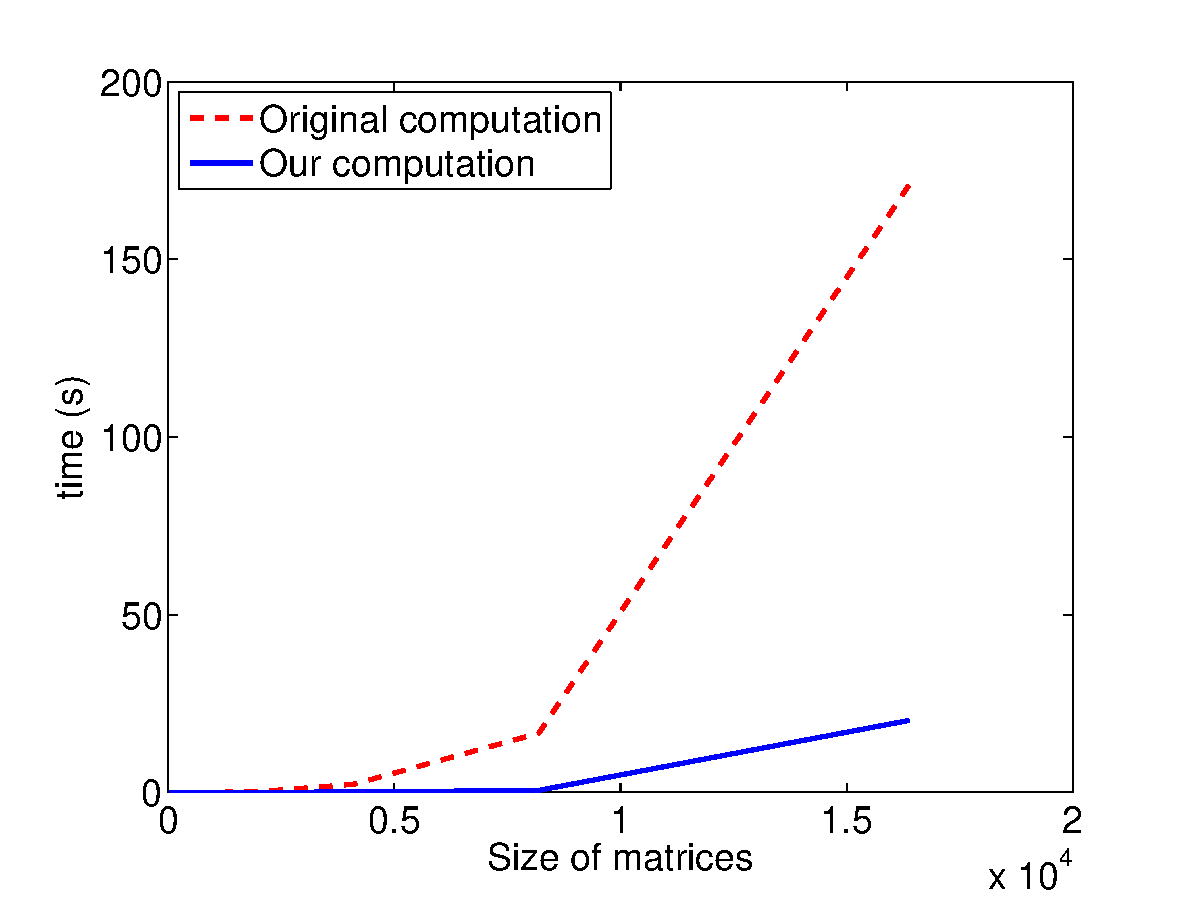
\includegraphics[width=0.55\linewidth]{img/ab.eps}
      \label{ab}
  }\quad
\subfigure[Approximations of $e^x$ using Taylor series.]{
  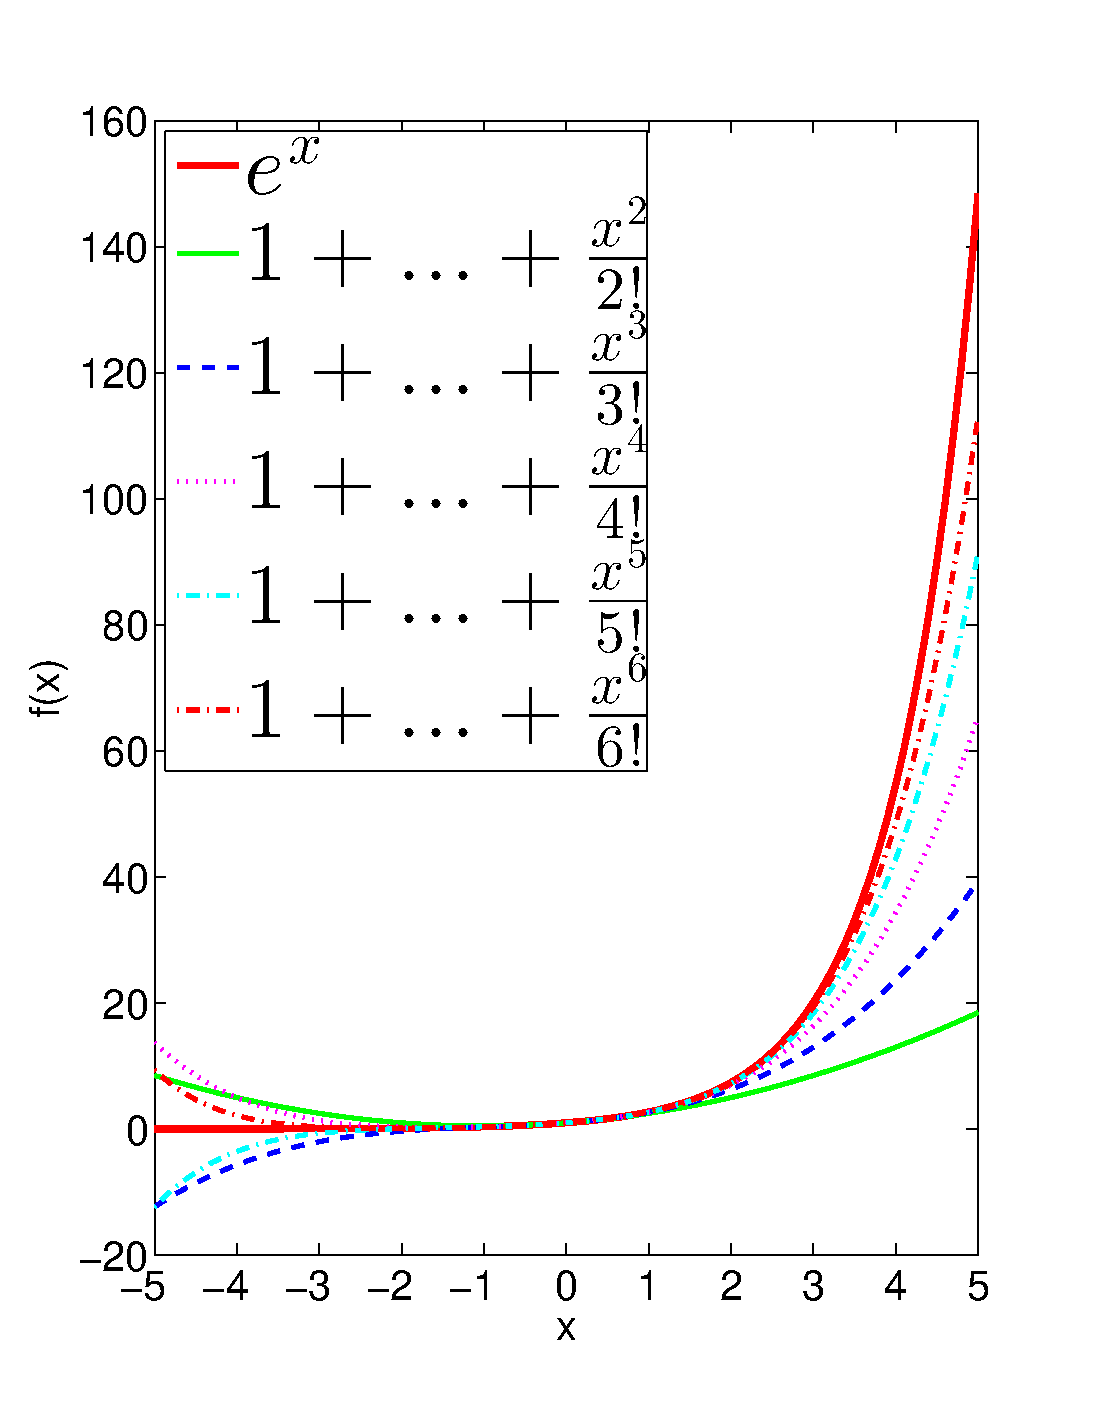
\includegraphics[width=0.35\linewidth]{img/approximations.eps} 
  \label{approximations}
  }
}
\vspace{-3mm}
\subfigure[Relative approximation error of the partition function for different
degrees of Taylor approximation. Max, mean and min errors are shown for 100
different trials for $W$ of size $ 7 \times 7$, with $W_{ij} \sim
\text{Laplacian}(s)$ and $s=0.05$ (blue) and $s=0.3$ (red).]{
  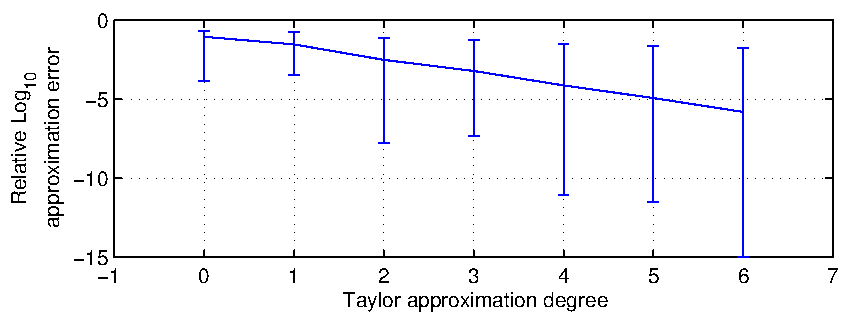
\includegraphics[scale=0.44]{img/partition_approx_rob.eps}
  \label{error_approx}
}

\subfigure[Comparison of computation time for naive exponential time algorithm vs our optimized derivation.]{
  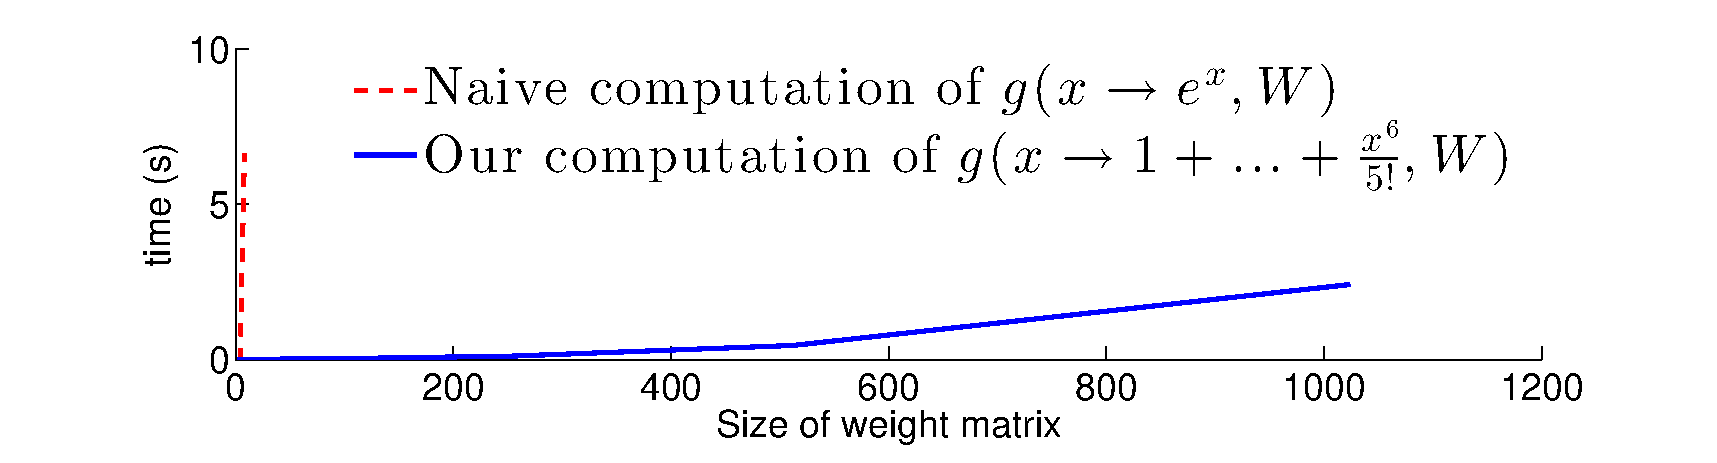
\includegraphics[scale=0.24]{img/time_approx.eps}
  \label{time_approx}
}
\vspace{-7mm}
\caption{Experimental results.}
\end{figure}

